\chapter{Introduction}

Our central problem is defined as follow:

% problem 1
\begin{problem}[Problem 1]:

Given a multi directed graph $G = (V, E)$ and a set of points of interest $V_P \subseteq V$.

Find $K$ closed walks that cover $V_P$.

\textbf{Objective:} Minimize the sum of walk length over all walks.

\textbf{Constraint 1:} Maximum walk length does not exceed $L$

\textbf{Constraint 2:} No overlap between any pair of walks.

\label{prob:problem1}
\end{problem}

Where a walk is defined as a sequence of edges (not necessary distinct). A closed walk is defined as a walk such that the starting node and the ending node are identical.


In order to solve the problem \ref{prob:problem1}, we introduce an equivalent problem as follow:

% problem 2
\begin{problem}[Problem 2]:

Given a directed graph $G_P = (V_P, E_P)$ with triangle equality.

Find $K$ cycles that cover $V_P$.

\textbf{Objective:} Minimize the sum of cycle length over all cycles.

\textbf{Constraint 1:} Maximum cycle length does not exceed $L$

\label{prob:problem2}
\end{problem}

Where a cycle is defined as a closed walk that all nodes are distinct.

% theorem 1
\begin{theorem}[Theorem 1]:


Problem \ref{prob:problem1}* (without constraint 2) and problem \ref{prob:problem2} can be reduced from each other.
\label{theo:theorem1}
\end{theorem}

Problem \ref{prob:problem1}* and problem \ref{prob:problem2} are equivalent. That means we can use the results of problem \ref{prob:problem2} to solve problem \ref{prob:problem1}* \footnote{Informal proof in Appendix}. The reduction is as follow:

% reduction 1
\begin{reduction}[problem \ref{prob:problem1}* $\to$ problem \ref{prob:problem2}]:


Given a multi directed graph $G = (V, E)$ and a set of points of interest $V_P \subseteq V$. Let $G_P = (V_P, E_P)$ be a directed graph such that each edge $(v_i, v_j) \in E_P$ is the shortest path in $G$.

\label{reduc:reduction1}
\end{reduction}

Using reduction \ref{reduc:reduction1}, we can construct an instance of problem \ref{prob:problem2} that is equivalent to problem \ref{prob:problem1}*. After solving $G_P$, we map each of the edges in the solution of $G_P$ by its corresponding shortest path in $G$.

\begin{figure}[h!]
\centering
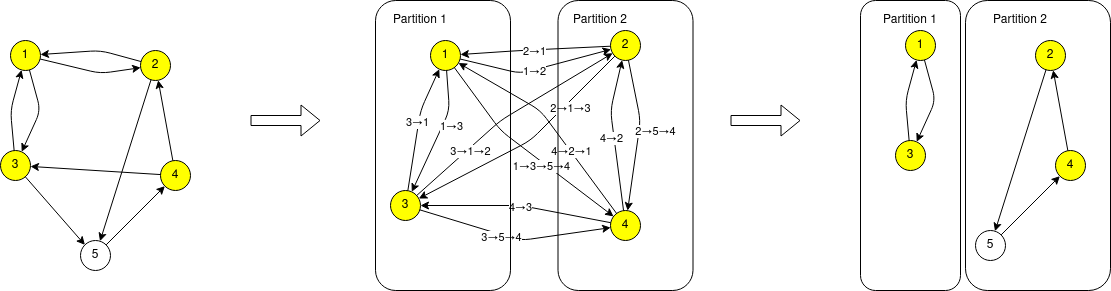
\includegraphics[width=0.8\textwidth]{assets/reduction.png}
\caption{Reduction}
\label{fig:reduction}
\end{figure}
